\documentclass[parskip=full]{scrartcl}
%\documentclass[a4paper]{article}
\usepackage[utf8]{inputenc} % use utf8 file encoding for TeX sources
\usepackage[T1]{fontenc}    % avoid garbled Unicode text in pdf
\usepackage[ngerman, english]{babel}  % german hyphenation, quotes, etc
\usepackage{graphicx}       % provides commands for including figures
\usepackage{rotating}	
\usepackage{amsmath}
\usepackage{amssymb}	
\graphicspath{ {images/} }
\usepackage{hyperref}       % detailed hyperlink/pdf configuration
\hypersetup{                % ‘texdoc hyperref‘ for options
	pdftitle={Proseminar : Matrix generator},%
	bookmarks=true
}
\usepackage{csquotes}       % provides \enquote{} macro for "quotes"
\usepackage[nonumberlist, acronym]{glossaries} % provides glossary commands
\usepackage{enumitem}
\usepackage{lscape}
\usepackage{caption}
\usepackage{placeins}


\begin{document}
	
	\begin{titlepage}
		\centering
		{\scshape\LARGE Karlsruher Institut für Technologie\par}
		\vspace{1cm}
		{\scshape\Large Final presentation\par}
		\vspace{1.5cm}
		{\huge\bfseries Automated test matrix generation\par}
		\vspace {2cm}
		
		{\Large\itshape Anna Katharina Ricker\par}
		
		\vfill
		Supervisors\par
		Hartwig Anzt
		Markus G\"{o}tz
		
		\vfill
		{\large\today\par}
	\end{titlepage}
	
	\tableofcontents
	\newpage
	
\section{Introduction}	
%more introduction!!
For the use case of generating matrices for training a neural network  classifying the best solver, it is important to have a large collection of matrices. When generating this matrices, it is not mandatory needed to generate a matrix with every tiny implementation option detailed chosen. 
It is rather useful to have many different matrices close to matrices representing real world problems. Because it was hard to find specific types of real world matrices, this generator is strongly oriented on LAPACK \cite{LAPACK}. LAPACK offers a random matrix generator, that was developed to generate matrices to test large numerical linear algebra libraries. 

\section{LAPACK}
LAPACK deals with the implementation of a suite of test matrix generators for testing linear algebra software. Their routines generate random matrices with certain properties which are useful for testing linear equation solving, least squares, and eigendecomposition software. These properties include the spectrum, symmetry, bandwidth, norm, sparsity, conditioning  (with respect to inversion or for the eigenproblem), type (real or complex), and storage scheme (dense, packed, or banded).
The three main routines LAPACK offers are called xLATMR, xLATMS and xLATME, where the first letter of each name (the `x') is either `S', `D', `C', or `Z'. 
\begin{itemize}
\item ‘S’ for single precision real (REAL)
\item ‘D’ for double precision real (DOUBLE PRECISION)
\item ‘C’ for single precision complex (COMPLEX)
\item ‘Z’ for double precision complex (DOUBLE COMPLEX)
\end{itemize}
Since complex matrices would go beyond the scope of what is needed for classification, this paper will focus on the LAPACK implementation of real matrices:

\newpage
\subsection{Distribution option in LAPACK}
LAPACK uses three different distributions:
\begin{itemize}
\item a uniform distribution on (0; 1)
\item a uniform distribution on (-1; 1)
\item a normal distribution with mean zero and variance one (normal(0; 1))
\end{itemize}

\subsection{Diagonalentries options in LAPACK}
To generate Diagonal entries, LAPACK always uses one of the following options:
\begin{itemize}
	\item Input by the user.
	\item D(1) = 1 and the other D(i)=1/COND, where COND >= 1 is a user input.
	\item D(N)=1/COND and the other D(i) = 1. 
	\item The D(i) form a geometric sequence from 1 to 1/COND. 
	\item The D(i) form an arithmetic sequence from 1 to 1/COND
	\item The D(i) are random in the range [1/COND; 1] with uniformly distributed logarithms. 
	\item The D(i) are random with the same distribution as the other matrix entries.
\end{itemize}

\subsection{Packing options in LAPACK}
The allowable options are: 
\begin{itemize}
\item no packing, 
\item zeroing out the upper or lower half (if symmetric or Hermitian), 
\item storing the upper or lower half columnwise (if symmetric, Hermitian or triangular), 
\item using triangular band storage (upper half or lower half, and only if the matrix is symmetric, Hermitian or triangular), and full band storage.
\end{itemize}

\subsection{The different generators in LAPACK}
\subsubsection{xLATMR}
xLATMR generates a matrix with random off-diagonal entries and given diagonal entries. It is the simplest (and fastest) of the three routines in the suite, and permits no direct control over the eigenvalues or singular values of the generated matrix.

\title hhigh level description:
\begin{enumerate}
\item Generate a matrix A with random entries with a distribution as described before in distribution-options
\item Set Diagonal of A to D where entries D are computed as explained before
\item Grade A, if desired, by pre- and postmultiplying it by diagonal matrices DL and DR, respectively. 
The entries of DL and DR are chosen just as the entries of D above
\item Permute the rows and columns of A, if desired.
\item Set random entries of A to zero, if desired, to get a matrix with a given fraction of zero entries.
\item Make A a band matrix, if desired, by zeroing out its entries outside given upper and lower bandwidths.
\item Scale A, if desired, to have a given maximum absolute entry.
\item Pack A, if desired
\end{enumerate}

\subsubsection{xLATMS}
xLATMS generates either a random real symmetric or complex Hermitian matrix with given eigenvalues and bandwidth, or a random nonsymmetric or complex symmetric matrix with given singular values and upper and lower bandwidth. 

\title hhigh level description:
\begin{enumerate}
	\item Set the diagonal of the matrix A to D, where the entries of D can be chosen as explained in chapter “Diagonalentrie options”. 
	The entries of D will be the eigenvalues (and/or singular values) of the final matrix.
	\item Pre- and postmultiply A by random orthogonal matrices (if A is real). 
	If A is to be symmetric, then the premultiplying matrix is the transpose of the postmultiplying one. 
	Otherwise, the pre- and postmultipying matrices are chosen independently of one another.
	\item Reduce A to have the desired bandwidth using Householder transformations.
	\item Pack A, if desired with the described packing-options
\end{enumerate}
For non-banded and large-bandwidth matrices, the preceding description accurately describes the procedure actually followed. For small-bandwidth matrices, steps 2-4 are replaced by a method which uses Givens rotations to increase the bandwidth to the desired value, rather than generating a dense matrix and then reducing its bandwidth. Givens rotation method is used, if:
\begin{itemize}
	\item the matrix is symmetric and the bandwidth (KL or KU) is less than N/2,
	\item the matrix is non-symmetric and KL + KU < 0,3(M + N) 
\end{itemize}
With KL being the lower bandwidth and KU the upper bandwidth.

\subsubsection{xLATME}
xLATME generates a random nonsymmetric matrix with given eigenvalues, either a given condition number for the eigenvalues or a given Jordan form (with certain restrictions), and a given one-sided bandwidth. Thus, for example, they can generate random Hessenberg matrices with given eigenvalues and sensitivities; this is useful for testing QR iteration algorithms for the nonsymmetric eigenproblem. Only dense storage is provided, since the nonsymmetric eigenroutines only work on matrices in dense storage format.

\title hhigh level description:
\begin{enumerate}
	\item Set the diagonal of the matrix A to D, where the entries of D can be chosen as explained in chapter “Diagonal-entry options”.
	
	\item If the user so specifies, the upper or lower triangle of A is filled with random numbers, which are chosen with a distribution described before in distribution options. 
	This option may be used to partially control the Jordan form of A as follows: 
	if A has any multiple eigenvalues and the upper triangle is filled in, then there will be exactly one Jordan block per distinct eigenvalue; such a matrix is called defective. 
	If the upper triangle is not filled in, there will only be 1 by 1 blocks in the Jordan form, even if there are multiple eigenvalues; such a matrix is called derogatory.
	
	\item If the user so specifies, A is premultiplied by a random matrix S and postmultiplied by S\textsuperscript{-1}. Here S is a random dense nonsymmetric matrix whose singular values DS may be chosen as described in “Diagonal-entry-options”. This option may be used to control the condition of A’s eigenproblem as follows: If the upper triangle has not been filled in, then the most sensitive eigenvalue of A will have sensitivity approximately equal to $\kappa  \equiv max_i |DS(i)|/min_i |DS(i)|$
	
	\item Where sensitivity means that a perturbation of norm $\varepsilon$ in A will cause a change an eigenvalue by a most approximately $ \kappa \cdot \varepsilon$ [6, 2]. 
	The approximation arises because the true sensitivity need only be within a factor N (the dimension of A) of the condition number of SX, where X is a diagonal matrix chosen so that the columns of SX have equal norm. In general, the columns of S will not differ too much in norm, so that the condition number of the eigenproblem may indeed be approximately controlled with this approach.
	
	\item If the user so specifies, either the upper or lower bandwidth (but not both) is reduced to any positive value desired.
	
	\item Scale A, if desired, to have a given maximum absolute entry.
\end{enumerate}

\newpage
\section{Automated test matrix generation}

The matrix generator should be easy to extend.  
That worked with defining different generator options similar as the LAPACK approach, which can be chosen by the user or will be selected randomly.
Therefore 6 matrix-generators and 6 diagonal-entry generators have been implemented.

\subsection{diagonal generator}
The approaches are adopted from LAPACK. But it is not possible to set diagonal entries by user input. That is why this generator has just 6 different diagonal entry setters:
\begin{enumerate}
	\item D(1) = 1 and the other D(i)=1/COND, where COND >= 1 is a user input.
	\item D(N)=1/COND and the other D(i) = 1. 
	\item The D(i) form a geometric sequence from 1 to 1/COND. 
	\item The D(i) form an arithmetic sequence from 1 to 1/COND
	\item The D(i) are random in the range [1/COND; 1] with uniformly distributed logarithms. 
	\item The D(i) are random with the same distribution as the other matrix entries.
\end{enumerate}
If the user input is defined by zero, a diagonal generator is randomly chosen.

\newpage
\subsection{Matrix generators}

\subsubsection{Generator 1}
\begin{figure}[h!]
	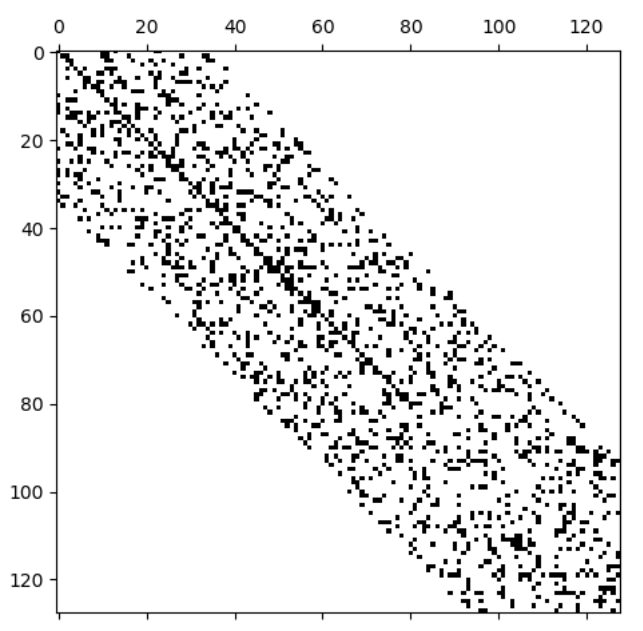
\includegraphics[width=0.5\textwidth]{images/g1_diag.PNG}
\end{figure}

This generator is based on xLATMS: 

\begin{enumerate}
	\item Set the diagonal of the matrix A to D, where the entries of D can be chosen as explained in chapter “Diagonal-entry options”. The entries of D will be the eigenvalues (and/or singular values) of the final matrix.
	\item Pre- and postmultiply A by random orthogonal matrices (if A is real). If A is to be symmetric, then the premultiplying matrix is the transpose of the postmultiplying one. Otherwise, the pre- and postmultiplying matrices are chosen independently of one another.
	\item Reduce A to have the desired bandwidth using Householder transformations \cite{numerikskript}.
	\item If desired lower the density. This step is not part of xLATMS, but in case of classification it is more useful to have a matrix with low density. 
\end{enumerate}

As it is useful to save all matrices from different generators and different types in one hdf5 file, there will be no packing options available in this approach.
To have an orthogonal matrix generator 1 can multiply matrix A with, generator 6 was added, that just creates orthogonal matrices.

\newpage
\subsubsection{Generator 2}
\begin{figure}[h!]
	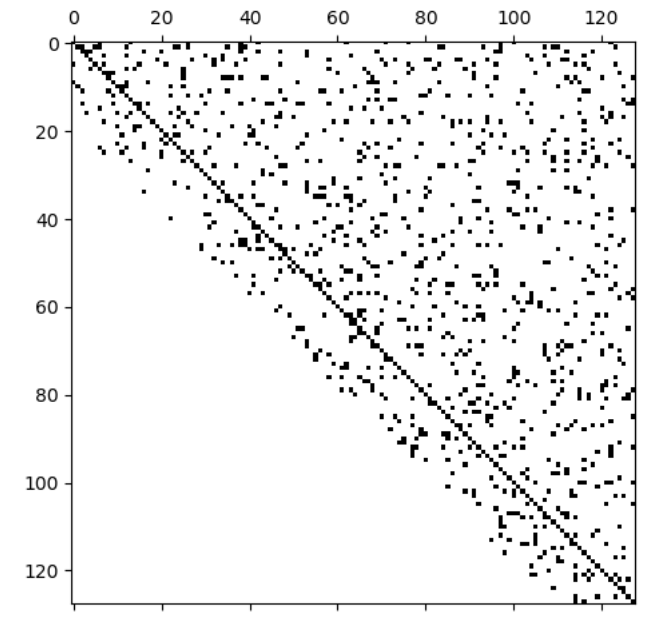
\includegraphics[width=0.5\textwidth]{images/g2_diag3.PNG}
\end{figure}
This generator is based on xLATME
\begin{enumerate}
	\item Set the diagonal of the matrix A to D, where the entries of D can be chosen as explained in chapter “Diagonal-entry options”.
	\item Fill randomly rather the upper, the lower or no triangle of matrix A.
	\item Randomly choose if matrix A will be multiplied by S and S\textsuperscript{-1} or not. S will be generated by generating random matrix entries with distributions as defined in Lapac. After that the diagonal-entries will be set by the diagonal-generator.
	This step is not part of xLatme, but it is similarity invariant, so by multiplying it keeps some important characteristics of matrix A.
	\item Randomly choose if the upper or lower bandwidth is reduced. The positive value is a random number between 1 and the size of the matrix with value = 1, meaning, A will be a triangular matrix.
	\item Randomly create the given density with the density setter. This step is also not part of xLATME but it causes a more slightly occupied matrix.
\end{enumerate}
Unlike to xLatme there is no possibility to scale the matrix. All matrix entries are always between -1 to 1 or 0 to 1.

\newpage
\subsubsection{Generator 3}
\begin{figure}[h!]
	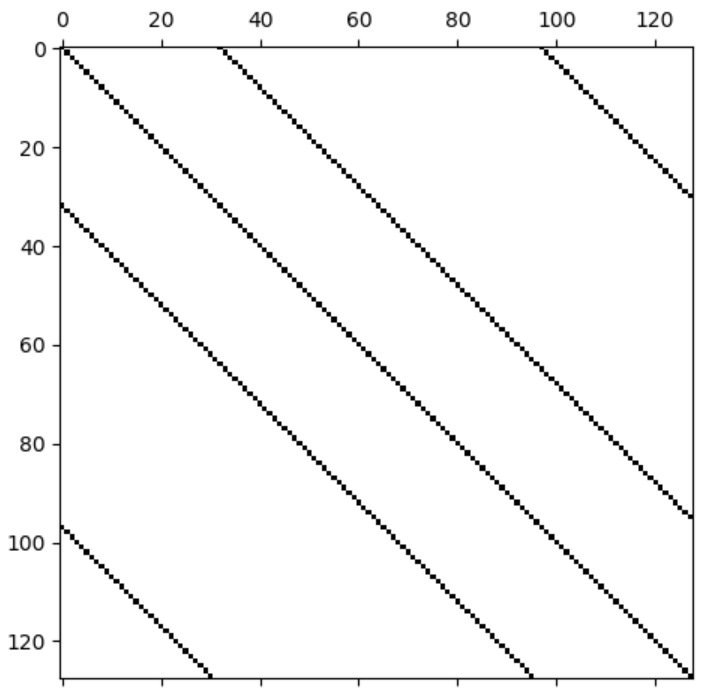
\includegraphics[width=0.5\textwidth]{images/Generator4.PNG}
\end{figure}
This generator deals with the topic of side diagonal matrices based on the problem of connectivity graphs, where the side diagonals of the matrix indicate the connectivity to other linear systems.
Generator 3 is not similar to any LAPACK generators. It just sets the diagonal entries with the diagonal entry generator. Following there will be 0 to 10 side diagonals with a randomly chosen distance filled with values unequal zero.
The distribution options for the random values are the same as given by LAPACK.

\newpage
\subsubsection{Generator 4}
\begin{figure}[h!]
	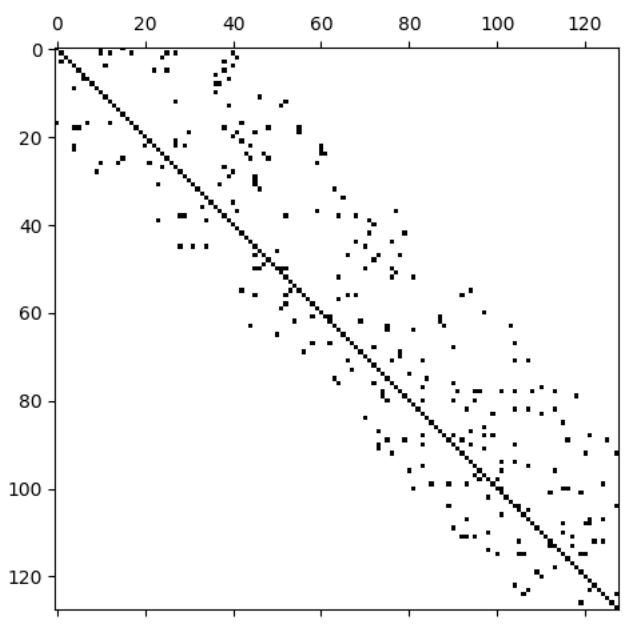
\includegraphics[width=0.5\textwidth]{images/g4_diag_dens_2.PNG}
\end{figure}
This generator is based on xLATMR:
\begin{enumerate}
	\item Spread random matrix entries all over the matrix with one of the distribution described before. to lower the density the density setter is also already used in this step.
	\item Randomly choose if a diagonal matrix will or will not be pre- or postmultiplied. The diagonal matrix is generated by the diagonal entry generator.
	\item Randomly choose if rows or columns will or will not be permuted.
	\item Randomly create the given density with the density setter.
	\item Randomly choose if the bandwidth is reduced. The positive value is a random number between 1 and the size of the matrix, with value = 1 meaning, A will be a diagonal matrix.
	\item Set diagonal entries at the end, so it is guaranteed, that the diagonal entries do not equal zero.
\end{enumerate}

\newpage
\subsubsection{Generator 5}
\begin{figure}[h!]
	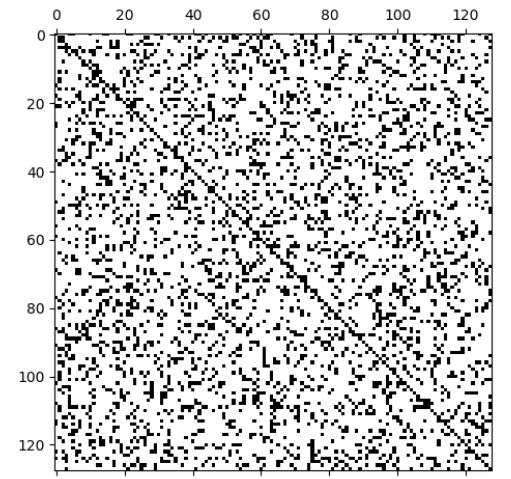
\includegraphics[width=0.5\textwidth]{images/g5_dens_diag.PNG}
\end{figure}
This generator does just generate orthogonal matrices. 
To generate an orthogonal matrix, the generator just creates a matrix with random value entries, that will in the next step be orthogonalised by Gram-Schmidt. Therefore the scipy library \cite{scipy} offers a function that constructs an orthonormal basis for the range of A using singular value decomposition of a matrix. 

\subsubsection{Generator 6}
\begin{figure}[h!]
	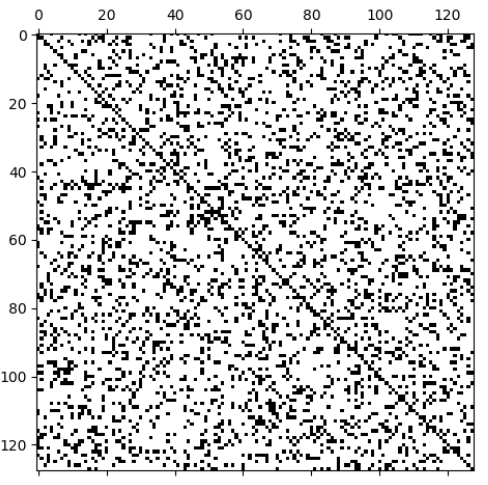
\includegraphics[width=0.5\textwidth]{images/g6_dens_diag.PNG}
\end{figure}
\newpage
This generator guarantees positive definite matrices.
By filling the diagonal entries with only positive entries and premultiplying with a matrix S and postmultiplying by S\textsuperscript{-1}
The multiplication result will be similar to the generated diagonal matrix which is positive definite. The multiplication by a matrix S and S\textsuperscript{-1} will be repeated 1 to 10 times randomly.

\subsection{Density setter}
To lower the density following steps will be made:
\begin{itemize}
	\item x = density * number of matrix entries
	\item Set random entries of A to zero (x times)
\end{itemize}
To guarantee that the main diagonal entries will not be zero, the diagonal entries will be set after spreading zeros to lower the density.


\subsection{Householder function}
The implementation of the householder function for reducing the bandwidth is based on the pseudocode out of "A Framework for Symmetric Band Reduction"\cite{Householder}. 
Using QR decomposition, different parts of matrix A are pre and postmultiplied by Q and Q\textsuperscript{T} multiple times.

\subsection{Regularity in matrix generation}
To use a matrix for training the neural network, the matrix has to be regular.
Not all of the generators guarantee generating a regular matrix, so the irregular matrices will be sorted out.
Generator 1 and 5 can guarantee regularity of all the generated matrices. An orthogonal matrix is always regular. 
Generator 1 multiplies a regular diagonal matrix with an orthogonal matrix, so in this step, the regularity will not get lost.
Even if transforming the matrix using the householder function, the regularity will remain.
Generator 2 and 4 cannot fully guarantee regularity because of the bandwidth reducing and the increasing of zero values to lower the density.
But both steps are randomly chosen and both steps do not necessarily ensure the matrix will loose its regularity.
Even for matrices generated by generator 3 it is rather unlikely that a diagonal matrix with just a few non zero side diagonals is not regular.
So the irregular matrices will just be sorted out.

\subsection{Positive definite matrix}
Analysing the trained neural network for classifying a matrix and looking at the different solver used for classification, brought up another interesting characteristic of a matrix for this use case: a few matrix should be positive definite.
Some solver work only or at least better on positive definite matrices. 
That is why generator 6 was created. 
The characteristic of a matrix being positive definite is similarity invariant. 
That means amongst other things, that premultiplying a positive definite matrix with a random matrix S and postmultiplying with S\textsuperscript{-1}, the result matrix will still be positive definite. 
So if the generator takes a diagonal matrix with just positive diagonal entries, the requirement, that the matrix is positive definite, is fulfilled.
Following the matrix can be pre and postmultiplied by S and S\textsuperscript{-1} as much as wanted. 

%\subsection{Random generator}

\subsection{User Input}
\begin{enumerate}
	\item matrix size: int
	\item density of the matrix: double [0, 1]
	\item positive definite: Boolean
	\item Distribution: 1-3
	\item amount of matrices: int
	\item storage location: String
	\item diagonal option: int between 1 and 6
	\item generation option: int between 1 and 6
	\item symmetric: boolean
\end{enumerate}

\newpage

\begin{thebibliography}{9}
	\bibitem{LAPACK} 
	James Demmel Alan McKenney. 
	\textit{LAPACK Working Note 9 ATest Matrix Generation Suite}. 
	
	\bibitem{numerikskript} 
	Marlis Hochbruck
	\textit{Numerische Mathematik I und II WS 2018/19 – SS 2019}. (German)  
	
	\bibitem{La}
	Kühnlein
	\textit{Lineare Algebra 2 skript} (German)
	
	\bibitem{Householder}
	Christian Bischof, Bruno Lang and Xiaobai Sun
	\textit{A Framework for Symmetric Band Reduction}
	
	\bibitem{scipy}
	Scipy library
	\\\texttt{https://docs.scipy.org/doc/scipy/}


\end{thebibliography}





\end{document}

